\documentclass[11pt, a4paper]{article}\usepackage[]{graphicx}\usepackage[]{xcolor}
% maxwidth is the original width if it is less than linewidth
% otherwise use linewidth (to make sure the graphics do not exceed the margin)
\makeatletter
\def\maxwidth{ %
  \ifdim\Gin@nat@width>\linewidth
    \linewidth
  \else
    \Gin@nat@width
  \fi
}
\makeatother

\definecolor{fgcolor}{rgb}{0.345, 0.345, 0.345}
\newcommand{\hlnum}[1]{\textcolor[rgb]{0.686,0.059,0.569}{#1}}%
\newcommand{\hlsng}[1]{\textcolor[rgb]{0.192,0.494,0.8}{#1}}%
\newcommand{\hlcom}[1]{\textcolor[rgb]{0.678,0.584,0.686}{\textit{#1}}}%
\newcommand{\hlopt}[1]{\textcolor[rgb]{0,0,0}{#1}}%
\newcommand{\hldef}[1]{\textcolor[rgb]{0.345,0.345,0.345}{#1}}%
\newcommand{\hlkwa}[1]{\textcolor[rgb]{0.161,0.373,0.58}{\textbf{#1}}}%
\newcommand{\hlkwb}[1]{\textcolor[rgb]{0.69,0.353,0.396}{#1}}%
\newcommand{\hlkwc}[1]{\textcolor[rgb]{0.333,0.667,0.333}{#1}}%
\newcommand{\hlkwd}[1]{\textcolor[rgb]{0.737,0.353,0.396}{\textbf{#1}}}%
\let\hlipl\hlkwb

\usepackage{framed}
\makeatletter
\newenvironment{kframe}{%
 \def\at@end@of@kframe{}%
 \ifinner\ifhmode%
  \def\at@end@of@kframe{\end{minipage}}%
  \begin{minipage}{\columnwidth}%
 \fi\fi%
 \def\FrameCommand##1{\hskip\@totalleftmargin \hskip-\fboxsep
 \colorbox{shadecolor}{##1}\hskip-\fboxsep
     % There is no \\@totalrightmargin, so:
     \hskip-\linewidth \hskip-\@totalleftmargin \hskip\columnwidth}%
 \MakeFramed {\advance\hsize-\width
   \@totalleftmargin\z@ \linewidth\hsize
   \@setminipage}}%
 {\par\unskip\endMakeFramed%
 \at@end@of@kframe}
\makeatother

\definecolor{shadecolor}{rgb}{.97, .97, .97}
\definecolor{messagecolor}{rgb}{0, 0, 0}
\definecolor{warningcolor}{rgb}{1, 0, 1}
\definecolor{errorcolor}{rgb}{1, 0, 0}
\newenvironment{knitrout}{}{} % an empty environment to be redefined in TeX

\usepackage{alltt}

\usepackage[top = 1 in, bottom = 1 in, left = 0.9 in, right = 0.9 in]{geometry}

\usepackage{amsmath, amssymb, amsfonts}
\usepackage{enumerate}
\usepackage{array}
\usepackage{multirow}
\usepackage{dingbat}
\usepackage{fontawesome5}
\usepackage{tasks}
\usepackage{bbding}
\usepackage{undertilde}
\usepackage{twemojis}
\usepackage{hyperref}
\usepackage{simpsons}
% how to use bull's eye ----- \scalebox{2.0}{\twemoji{bullseye}}
\usepackage{fontspec}
\usepackage{customdice}
% how to put dice face ------ \dice{2}

\title{MSMS 206 : Practical 11}
\author{Ananda Biswas}
\date{\today}

\newfontface\myfont{Myfont1-Regular.ttf}[LetterSpace=0.05em]
% how to use ---- {\setlength{\spaceskip}{1em plus 0.5em minus 0.5em} \fontsize{17}{20}\myfont --write text here-- \par}

\newfontface\cbfont{CaveatBrush-Regular.ttf}
% how to use --- \myfont --write text here--
\IfFileExists{upquote.sty}{\usepackage{upquote}}{}
\begin{document}

\maketitle


\scalebox{2.0}{\twemoji{bullseye}} \hspace{0.2cm} \textcolor{blue}{\textbf{Question : }} Write a program to generate random sample from Poisson Process with parameter $\lambda$. \\[0.5em]

Also write programs to generate $X(t)$ if 

\begin{enumerate}[(a)]

\item ${\displaystyle P(X(t) = k) = \binom{k + \alpha - 1}{k} \left( \dfrac{\beta}{t+\beta} \right)^{\alpha} \left( \dfrac{t}{t+\beta} \right)^k ; \,\,\, k = 0, 1, 2, \ldots}$.

\item $P(X(t) = k) = \left( \dfrac{t}{t+\mu} \right)^k \left( \dfrac{\mu}{t+\mu} \right); \,\,\, k = 0, 1, 2, \ldots$.

\end{enumerate}

\vspace{0.2cm}

\faArrowAltCircleRight[regular] \hspace{0.2cm} \underline{A realization of Poisson Process}\\[1em]

We take $\lambda = 2$ and observe the Poisson Process upto time $T = 5$.

\begin{knitrout}
\definecolor{shadecolor}{rgb}{0.969, 0.969, 0.969}\color{fgcolor}\begin{kframe}
\begin{alltt}
\hldef{T} \hlkwb{<-} \hlnum{5}

\hldef{lambda} \hlkwb{<-} \hlnum{2}
\end{alltt}
\end{kframe}
\end{knitrout}

We observe the arrival times upto time $T$, for that we generate exponentially distributed random numbers with rate $\lambda$ until total time becomes $T$. The count of the arrival times form a realization of a Poisson Process with parameter $\lambda$.

\begin{knitrout}
\definecolor{shadecolor}{rgb}{0.969, 0.969, 0.969}\color{fgcolor}\begin{kframe}
\begin{alltt}
\hldef{times} \hlkwb{<-} \hlkwd{c}\hldef{(}\hlnum{0}\hldef{)}

\hldef{i} \hlkwb{<-} \hlnum{2}

\hldef{sum_times} \hlkwb{<-} \hlnum{0}

\hlkwa{while}\hldef{(sum_times} \hlopt{<} \hldef{T)\{}

  \hldef{times[i]} \hlkwb{<-} \hlkwd{round}\hldef{(}\hlkwd{rexp}\hldef{(}\hlnum{1}\hldef{,} \hlkwc{rate} \hldef{= lambda),} \hlkwc{digits} \hldef{=} \hlnum{2}\hldef{)}

  \hldef{sum_times} \hlkwb{<-} \hlkwd{sum}\hldef{(times)}

  \hldef{i} \hlkwb{<-} \hldef{i} \hlopt{+} \hlnum{1}
\hldef{\}}

\hldef{occurrence_times} \hlkwb{<-} \hlkwd{cumsum}\hldef{(times[}\hlopt{-}\hlkwd{length}\hldef{(times)])}

\hldef{x} \hlkwb{<-} \hlnum{0}\hlopt{:}\hldef{(}\hlkwd{length}\hldef{(occurrence_times)}\hlopt{-}\hlnum{1}\hldef{)}
\end{alltt}
\end{kframe}
\end{knitrout}

\begin{knitrout}
\definecolor{shadecolor}{rgb}{0.969, 0.969, 0.969}\color{fgcolor}\begin{kframe}
\begin{alltt}
\hldef{df1} \hlkwb{<-} \hlkwd{data.frame}\hldef{(}\hlkwc{States} \hldef{= x,} \hlkwc{Occurrence_Time} \hldef{= occurrence_times)}
\end{alltt}
\end{kframe}
\end{knitrout}

\smallpencil {\setlength{\spaceskip}{1em plus 0.5em minus 0.5em} \fontsize{17}{20}\myfont States and their arrival times are as follows : \par}

\begin{knitrout}
\definecolor{shadecolor}{rgb}{0.969, 0.969, 0.969}\color{fgcolor}\begin{kframe}
\begin{alltt}
\hldef{df1}
\end{alltt}
\begin{verbatim}
##    States Occurrence_Time
## 1       0            0.00
## 2       1            0.09
## 3       2            0.74
## 4       3            0.83
## 5       4            2.51
## 6       5            2.62
## 7       6            3.36
## 8       7            4.13
## 9       8            4.17
## 10      9            4.39
## 11     10            4.47
## 12     11            4.62
## 13     12            4.85
\end{verbatim}
\end{kframe}
\end{knitrout}

\smallpencil {\setlength{\spaceskip}{1em plus 0.5em minus 0.5em} \fontsize{17}{20}\myfont A realization of a Poisson Process with $\lambda = 2$ in $(0, 5]$ is as follows : \par}

$$X(t) = 
\begin{cases}
0, & \text{if } 0 \leq t < 0 \\
1, & \text{if } 0 \leq t < 0.09 \\
2, & \text{if } 0.09 \leq t < 0.74 \\
\vdots & \vdots \\
11, & \text{if } 4.62 \leq t < 4.85 \\
12, & \text{if } 4.85 \leq t \leq 5
\end{cases}$$

\newpage

\faArrowAltCircleRight[regular] \hspace{0.2cm} \underline{Visualization}

\begin{knitrout}
\definecolor{shadecolor}{rgb}{0.969, 0.969, 0.969}\color{fgcolor}\begin{kframe}
\begin{alltt}
\hlkwd{plot}\hldef{(}\hlkwd{c}\hldef{(x, x[}\hlkwd{length}\hldef{(x)])} \hlopt{~} \hlkwd{c}\hldef{(occurrence_times, T),}
     \hlkwc{type} \hldef{=} \hlsng{"s"}\hldef{,}
     \hlkwc{col} \hldef{=} \hlsng{"blue"}\hldef{,}
     \hlkwc{xaxt} \hldef{=} \hlsng{"n"}\hldef{,}
     \hlkwc{yaxt} \hldef{=} \hlsng{"n"}\hldef{,}
     \hlkwc{xlim} \hldef{=} \hlkwd{c}\hldef{(}\hlnum{0}\hldef{, T} \hlopt{+} \hlnum{0.05}\hldef{),}
     \hlkwc{xlab} \hldef{=} \hlsng{"Occurrence Time"}\hldef{,}
     \hlkwc{ylab} \hldef{=} \hlsng{"State"}\hldef{,}
     \hlkwc{main} \hldef{=} \hlkwd{paste}\hldef{(}\hlsng{"Realization of Poisson Process with lambda = "}\hldef{, lambda))}

\hlkwd{axis}\hldef{(}\hlnum{1}\hldef{,} \hlkwc{at} \hldef{= occurrence_times,} \hlkwc{labels} \hldef{= occurrence_times,} \hlkwc{las} \hldef{=} \hlnum{2}\hldef{)}
\hlkwd{axis}\hldef{(}\hlnum{2}\hldef{,} \hlkwc{at} \hldef{= x,} \hlkwc{labels} \hldef{= x)}
\hlkwd{points}\hldef{(occurrence_times, x,} \hlkwc{cex} \hldef{=} \hlnum{1}\hldef{,} \hlkwc{col} \hldef{=} \hlsng{"blue"}\hldef{,} \hlkwc{pch} \hldef{=} \hlnum{19}\hldef{)}
\hlkwd{abline}\hldef{(}\hlkwc{v} \hldef{= T,} \hlkwc{col} \hldef{=} \hlsng{"red"}\hldef{)}
\end{alltt}
\end{kframe}
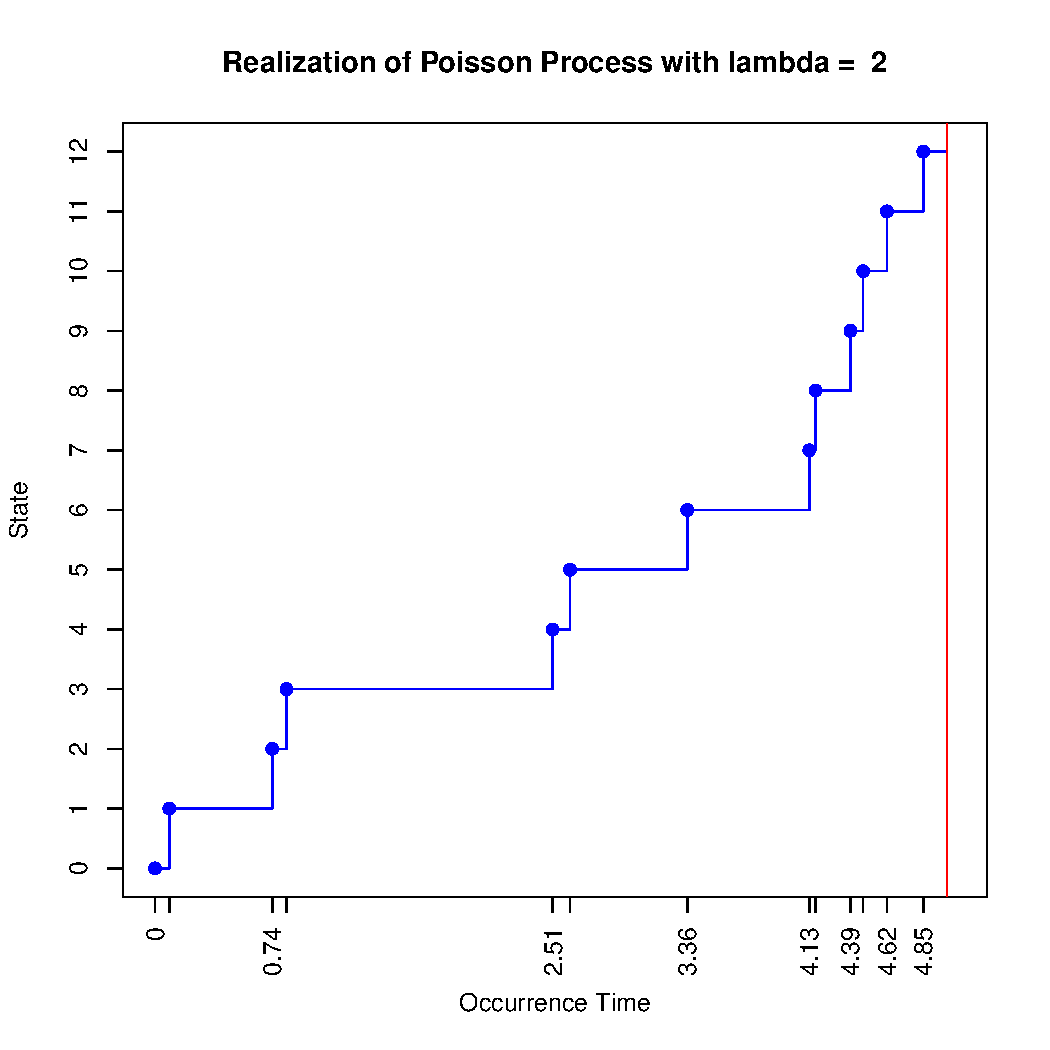
\includegraphics[width=\maxwidth]{figure/unnamed-chunk-5-1} 
\end{knitrout}


\faArrowAltCircleRight[regular] \hspace{0.2cm} \underline{$X(t) \sim $ Negative Binomial}\\[1em]

${\displaystyle P(X(t) = k) = \binom{k + \alpha - 1}{k} \left( \dfrac{\beta}{t+\beta} \right)^{\alpha} \left( \dfrac{t}{t+\beta} \right)^k ; \,\,\, k = 0, 1, 2, \ldots}$ \\

\vspace{0.2cm}

\textit{i.e.} $X(t) \sim \text{Negative Binomial}\left( \alpha, \dfrac{\beta}{t + \beta} \right)$. \\

\vspace{0.2cm}

Previously $\lambda$ was a fixed parameter. Now $\lambda$ will be sampled from $\text{Gamma}(\text{shape} = \alpha, \text{rate} = \beta).$

Here we take $\alpha = 2$, $\beta = 1$.

\begin{knitrout}
\definecolor{shadecolor}{rgb}{0.969, 0.969, 0.969}\color{fgcolor}\begin{kframe}
\begin{alltt}
\hldef{alpha} \hlkwb{<-} \hlnum{2}\hldef{; beta} \hlkwb{<-} \hlnum{1}
\end{alltt}
\end{kframe}
\end{knitrout}

\begin{knitrout}
\definecolor{shadecolor}{rgb}{0.969, 0.969, 0.969}\color{fgcolor}\begin{kframe}
\begin{alltt}
\hldef{T} \hlkwb{<-} \hlnum{5}

\hldef{lambda} \hlkwb{<-} \hlkwd{rgamma}\hldef{(}\hlnum{1}\hldef{,} \hlkwc{shape} \hldef{= alpha,} \hlkwc{rate} \hldef{= beta)}
\end{alltt}
\end{kframe}
\end{knitrout}

\begin{knitrout}
\definecolor{shadecolor}{rgb}{0.969, 0.969, 0.969}\color{fgcolor}\begin{kframe}
\begin{alltt}
\hldef{times} \hlkwb{<-} \hlkwd{c}\hldef{(}\hlnum{0}\hldef{)}

\hldef{i} \hlkwb{<-} \hlnum{2}

\hldef{sum_times} \hlkwb{<-} \hlnum{0}

\hlkwa{while}\hldef{(sum_times} \hlopt{<} \hldef{T)\{}

  \hldef{times[i]} \hlkwb{<-} \hlkwd{round}\hldef{(}\hlkwd{rexp}\hldef{(}\hlnum{1}\hldef{,} \hlkwc{rate} \hldef{= lambda),} \hlkwc{digits} \hldef{=} \hlnum{2}\hldef{)}

  \hldef{sum_times} \hlkwb{<-} \hlkwd{sum}\hldef{(times)}

  \hldef{i} \hlkwb{<-} \hldef{i} \hlopt{+} \hlnum{1}
\hldef{\}}

\hldef{occurrence_times} \hlkwb{<-} \hlkwd{cumsum}\hldef{(times[}\hlopt{-}\hlkwd{length}\hldef{(times)])}

\hldef{x} \hlkwb{<-} \hlnum{0}\hlopt{:}\hldef{(}\hlkwd{length}\hldef{(occurrence_times)}\hlopt{-}\hlnum{1}\hldef{)}
\end{alltt}
\end{kframe}
\end{knitrout}

\begin{knitrout}
\definecolor{shadecolor}{rgb}{0.969, 0.969, 0.969}\color{fgcolor}\begin{kframe}
\begin{alltt}
\hldef{df2} \hlkwb{<-} \hlkwd{data.frame}\hldef{(}\hlkwc{States} \hldef{= x,} \hlkwc{Occurrence_Time} \hldef{= occurrence_times)}
\end{alltt}
\end{kframe}
\end{knitrout}

\begin{knitrout}
\definecolor{shadecolor}{rgb}{0.969, 0.969, 0.969}\color{fgcolor}\begin{kframe}
\begin{alltt}
\hldef{df2}
\end{alltt}
\begin{verbatim}
##   States Occurrence_Time
## 1      0            0.00
## 2      1            0.26
## 3      2            1.67
\end{verbatim}
\end{kframe}
\end{knitrout}


\newpage

\faArrowAltCircleRight[regular] \hspace{0.2cm} \underline{$ X(t) \sim $ Geometric}\\[1em]

$P(X(t) = k) = \left( \dfrac{t}{t+\mu} \right)^k \left( \dfrac{\mu}{t+\mu} \right); \,\,\, k = 0, 1, 2, \ldots$ \textit{i.e.} $X(t) \sim \text{Geometric} \left( \dfrac{\mu}{t+\mu} \right). $ \\

\vspace{0.2cm}

Previously $\lambda$ was a fixed parameter. Now $\lambda$ will be sampled from $\text{Gamma}(\text{shape} = 1, \text{rate} = \mu) \Leftrightarrow \text{Exp}(\text{rate} = \mu).$

Here we take $\mu = 2$.

\begin{knitrout}
\definecolor{shadecolor}{rgb}{0.969, 0.969, 0.969}\color{fgcolor}\begin{kframe}
\begin{alltt}
\hldef{mu} \hlkwb{<-} \hlnum{2}
\end{alltt}
\end{kframe}
\end{knitrout}

\begin{knitrout}
\definecolor{shadecolor}{rgb}{0.969, 0.969, 0.969}\color{fgcolor}\begin{kframe}
\begin{alltt}
\hldef{T} \hlkwb{<-} \hlnum{5}

\hldef{lambda} \hlkwb{<-} \hlkwd{rgamma}\hldef{(}\hlnum{1}\hldef{,} \hlkwc{shape} \hldef{=} \hlnum{1}\hldef{,} \hlkwc{rate} \hldef{= mu)}
\end{alltt}
\end{kframe}
\end{knitrout}

\begin{knitrout}
\definecolor{shadecolor}{rgb}{0.969, 0.969, 0.969}\color{fgcolor}\begin{kframe}
\begin{alltt}
\hldef{times} \hlkwb{<-} \hlkwd{c}\hldef{(}\hlnum{0}\hldef{)}

\hldef{i} \hlkwb{<-} \hlnum{2}

\hldef{sum_times} \hlkwb{<-} \hlnum{0}

\hlkwa{while}\hldef{(sum_times} \hlopt{<} \hldef{T)\{}

  \hldef{times[i]} \hlkwb{<-} \hlkwd{round}\hldef{(}\hlkwd{rexp}\hldef{(}\hlnum{1}\hldef{,} \hlkwc{rate} \hldef{= lambda),} \hlkwc{digits} \hldef{=} \hlnum{2}\hldef{)}

  \hldef{sum_times} \hlkwb{<-} \hlkwd{sum}\hldef{(times)}

  \hldef{i} \hlkwb{<-} \hldef{i} \hlopt{+} \hlnum{1}
\hldef{\}}

\hldef{occurrence_times} \hlkwb{<-} \hlkwd{cumsum}\hldef{(times[}\hlopt{-}\hlkwd{length}\hldef{(times)])}

\hldef{x} \hlkwb{<-} \hlnum{0}\hlopt{:}\hldef{(}\hlkwd{length}\hldef{(occurrence_times)}\hlopt{-}\hlnum{1}\hldef{)}
\end{alltt}
\end{kframe}
\end{knitrout}

\begin{knitrout}
\definecolor{shadecolor}{rgb}{0.969, 0.969, 0.969}\color{fgcolor}\begin{kframe}
\begin{alltt}
\hldef{df3} \hlkwb{<-} \hlkwd{data.frame}\hldef{(}\hlkwc{States} \hldef{= x,} \hlkwc{Occurrence_Time} \hldef{= occurrence_times)}
\end{alltt}
\end{kframe}
\end{knitrout}

\begin{knitrout}
\definecolor{shadecolor}{rgb}{0.969, 0.969, 0.969}\color{fgcolor}\begin{kframe}
\begin{alltt}
\hldef{df3}
\end{alltt}
\begin{verbatim}
##   States Occurrence_Time
## 1      0            0.00
## 2      1            0.72
## 3      2            3.23
## 4      3            3.50
## 5      4            4.80
\end{verbatim}
\end{kframe}
\end{knitrout}


\end{document}
